\documentclass{article}
\setlength{\parskip}{0pt} % esp. entre parrafos
\setlength{\parindent}{20pt} % esp. al inicio de un parrafo
\usepackage{amsmath} % mates
\usepackage{listings}
\usepackage{xcolor}
\usepackage[sort&compress,numbers]{natbib} % referencias
\usepackage{url} % que las URLs se vean lindas
\usepackage[top=10mm,left=20mm,right=20mm,bottom=25mm]{geometry} % \textbf{\textbf{}}margenes
\usepackage{hyperref} % ligas de URLs
\usepackage{graphicx} % poner figuras
\usepackage{caption}
\usepackage{subcaption}
\usepackage[spanish]{babel} % otros idiomas
\hypersetup{
    colorlinks=true,
    linkcolor=blue,
    filecolor=blue,      
    urlcolor=blue,
}
\renewcommand{\lstlistingname}{C\'odigo}
\definecolor{codegreen}{rgb}{0,0.6,0}
\definecolor{codegray}{rgb}{0.5,0.5,0.5}
\definecolor{codepurple}{rgb}{0.58,0,0.82}
\definecolor{backcolour}{rgb}{0.95,0.95,0.92}
\lstdefinestyle{mystyle}{
    backgroundcolor=\color{backcolour},   
    commentstyle=\color{codegreen},
    keywordstyle=\color{magenta},
    numberstyle=\tiny\color{codegray},
    stringstyle=\color{codepurple},
    basicstyle=\ttfamily\footnotesize,
    breakatwhitespace=false,         
    breaklines=true,                 
    keepspaces=true,                 
    numbers=left,                    
    numbersep=5pt,                  
    showspaces=false,                
    showstringspaces=false,
    showtabs=false,                  
    tabsize=2
}

\lstset{style=mystyle}

\title{Reporte 10:\\Algoritmo Gen\'etico}
\author{Jorge Torres}
\date{\today}

\begin{document}

\maketitle

\section{Objetivo}\label{obj}
El problema de la mochila (ingl\'es: knapsack) es un problema cl\'asico de optimización, particularmente de programaci\'on entera, donde la tarea consiste en seleccionar un subconjunto de objetos de tal forma que (i) no se exceda la capacidad de la mochila en t\'erminos de la suma de los pesos de los objetos incluidos, y que (ii) el valor total de los objetos incluidos sea lo máximo posible. Este problema es pseudo-polinomial, ya que existe un \href{https://github.com/satuelisa/Simulation/blob/master/GeneticAlgorithm/knapsack.py}{algoritmo} de tabulaci\'on que determina la combinación óptima.\\

Un algoritmo genético representa posibles soluciones a un problema en términos de un genoma, que en este caso va a ser un vector de verdades y falsos, indicando cuáles objetos se van a incluir en la mochila (\texttt{TRUE} o 1 significa que llevamos el objeto, \texttt{FALSE} o 0 que lo descartamos de la selección).\\

El objetivo de esta actividad consiste en generar tres instancias con tres distintas reglas:

\begin{itemize}
    \item Instancia 1: el peso y el valor de cada objeto se generan independientemente con una distribución uniforme.
    \item Instancia 2: el valor de cada objeto se genera independientemente con una distribución exponencial y su peso es inversamente correlacionado con el valor.
    \item Instancia 3: el peso de cada objeto se genera independientemente con una distribución normal y su valor es (positivamente) correlacionado con el cuadrado del peso, con un ruido normalmente distribuido de baja magnitud.
\end{itemize}

\section{Desarrollo}

El desarrollo de la actividad est\'a basado en el \href{https://github.com/satuelisa/Simulation/blob/master/GeneticAlgorithm/perfGA.py}{c\'odigo} implementado por E. Schaeffer, en el que primero calcula el \'optimo te\'orico del problema de la mochila y despu\'es lo compara con los resultados del algoritmo gen\'etico \cite{elisa1}. La funci\'on \texttt{knapsack()} del c\'odigo \ref{codigo1} calcula el \'optimo te\'orico del problema pseudo-polinomial. El desarrollo completo puede encontrarse en el repositorio en GitHub de J. Torres \cite{jorge1}.

\begin{lstlisting}[caption=Soluci\'on \'Optima, label=codigo1, language=Python]
def knapsack(peso_permitido, pesos, valores):
    assert len(pesos) == len(valores)
    peso_total = sum(pesos)
    valor_total = sum(valores)
    if peso_total < peso_permitido: 
        return valor_total
    else:
        V = dict()
        for w in range(peso_permitido + 1):
            V[(w, 0)] = 0
        for i in range(len(pesos)):
            peso = pesos[i]
            valor = valores[i]
            for w in range(peso_permitido + 1):
                cand = V.get((w - peso, i), -float('inf')) + valor
                V[(w, i + 1)] = max(V[(w, i)], cand)
        return max(V.values())
\end{lstlisting}

Las funciones \texttt{factible()} y \texttt{objetivo()} del c\'odigo \ref{codigo2} determinan si el peso de los objetos seleccionados es menor al l\'imite y el valor total de dichos objetos, respectivamente.

\begin{lstlisting}[caption=Peso y Valor Totales de la Selecci\'on, label=codigo2, language=Python]
def factible(seleccion, pesos, capacidad):
    return np.inner(seleccion, pesos) <= capacidad
  
def objetivo(seleccion, valores):
    return np.inner(seleccion, valores)
\end{lstlisting}

En el c\'odigo \ref{codigo3} se tienen cuatro funciones. La funci\'on \texttt{normalizar()} arregla una distribuci\'on entre 0 y 1 de un conjunto de datos, que se utiliza para obtener valores aleatorios con esta distribuci\'on en subsecuentes funciones. La funci\'on \texttt{poblacion\_inicial()} crea un arreglo bidimensional de $n$ columnas (objetos) y $tam$ filas (individuos) con $n$ valores 0 \'o 1 aleatoria e uniformemente distribu\'idos para cada individuo. La funci\'on \texttt{mutacion()} selecciona objetos al azar de los individuos y, si el valor actual es 0, lo cambia a 1, creando un individuo diferente. La funci\'on \texttt{reproduccion()} toma dos individuos, selecciona una posici\'on al azar en sus vectores de objetos, y la utiliza como posici\'on de corte. Despu\'es realiza un cruzamiento entre los vectores cortados, creando un nuevo individuo que tiene informaci\'on de los individuos originales.

\begin{lstlisting}[caption={Funciones Normalizar, Poblaci\'on Inicial, Mutaci\'on y Reproducci\'on}, label=codigo3, language=Python]
def normalizar(data):
    menor = min(data)
    mayor = max(data)
    rango  = mayor - menor
    data = data - menor # > 0
    return data / rango # entre 0 y 1

def poblacion_inicial(n, tam):
    pobl = np.zeros((tam, n))
    for i in range(tam):
        pobl[i] = (np.round(np.random.uniform(size = n))).astype(int)
    return pobl

def mutacion(sol, n):
    pos = randint(0, n - 1)
    mut = np.copy(sol)
    mut[pos] = 1 if sol[pos] == 0 else 0
    return mut

def reproduccion(x, y, n):
    pos = randint(2, n - 2)
    xy = np.concatenate([x[:pos], y[pos:]])
    yx = np.concatenate([y[:pos], x[pos:]])
    return (xy, yx)
\end{lstlisting}

Para realizar observaciones basadas en las instancias mencionadas en la secci\'on \ref{obj}, se incluyen un total de 6 generadores de pesos y valores aleatorios, cuyos c\'odigos se discuten en las siguientes secciones.

\subsection{Generadores - Instancia 1}

En el c\'odigo \ref{codigo4}, con las funci\'ones \texttt{generador\_pesos()} y \texttt{generador\_valores()} se generan independientemente una cantidad $n$ de pesos y valores de manera aleatoria y uniformemente distribu\'idos.

\begin{lstlisting}[caption={Generadores de Pesos y Valores de Instancia 1}, label=codigo4, language=Python]
def generador_pesos(cuantos, low, high):
    return np.round(normalizar(np.random.uniform(low=low, high=high, size = cuantos)) * (high - low) + low)
 
def generador_valores(pesos, low, high):
    return np.round(normalizar(np.random.uniform(low = low, high = high, size = pesos)) * (high - low) + low)
\end{lstlisting}

\subsection{Generadores - Instancia 2}

La funci\'on \texttt{generador\_valores2()} del c\'odigo \ref{codigo5} crea aleatoriamente una cantidad $n$ de valores con una distribuci\'on exponencial, mientras que la funci\'on \texttt{generador\_pesos2()} obtiene la misma cantidad de pesos cuyo valor num\'erico est\'a correlacionado con el inverso de los valores.

\newpage

\begin{lstlisting}[caption={Generadores de Pesos y Valores de Instancia 2}, label=codigo5, language=Python]
def generador_pesos2(valores, low, high):
    cant = 1 / valores
    return np.round(((normalizar(cant))) * (high - low) + low)
 
def generador_valores2(pesos, low, high):
    cant = np.arange(0, pesos)  
    return np.round(normalizar(expon.pdf(cant))  * (high - low) + low)
\end{lstlisting}

\subsection{Generadores - Instancia 3}

En la tercera instancia, se necesitan obtener pesos independientemente con una distribuci\'on normal, mietras que los valores est\'an positivamente correlacionados con el cuadrado de los pesos, lo cual se implementa con las funciones \texttt{generador\_pesos3()} y \texttt{generador\_valores3()} del c\'odigo \ref{codigo6}.

\begin{lstlisting}[caption={Generadores de Pesos y Valores de Instancia 3}, label=codigo6, language=Python]
def generador_pesos3(cuantos, low, high):
    return np.round(normalizar(np.random.normal(size = cuantos)) * (high - low) + low)

def generador_valores3(pesos, low, high):
    return np.round((pesos**2) * (high - low) + low)
\end{lstlisting}

\newblock

Para las tres instancias se crean $n=100$ pesos y valores, el algoritmo se itera en 150 pasos y se realizan 20 repeticiones de cada instancia. Sin embargo, se hacen dos combinaciones distintas variando la probabilidad de mutaci\'on, la cantidad de reproducciones o cruzamientos, y la poblaci\'on inicial de individuos. La primera combinaci\'on consiste en una probabilidad de mutaci\'on $pm=0.05$, una cantidad de cruzamientos $rep=50$ y una poblaci\'on inicial $init=100$. La segunda combinaci\'on consiste en $pm=0.1$, $rep=100$ e $init=50$. Estos par\'ametros se pueden observar en el c\'odigo \ref{codigo7}.

\begin{lstlisting}[caption={Par\'ametros Iniciales}, label=codigo7, language=Python]
n = 100
tmax = 150
iteraciones = 20

#####Combinacion 1#####

pm, rep, init = 0.05, 50, 100

#####Combinacion 2#####

pm, rep, init = 0.1, 100, 50
\end{lstlisting}

Al iniciar las iteraciones, se generan los pesos y valores, se define la capacidad m\'axima de la mochila, se calcula el valor \'optimo con la funci\'on \texttt{knapsack()} y se crea la poblaci\'on inicial de individuos, como se observa en el c\'odigo \ref{codigo8}.

\begin{lstlisting}[caption=Inicio de Iteraciones, label=codigo8, language=Python]
for runs in range(iteraciones):
    pesos = generador_pesos(n, 15, 80)
    valores = generador_valores(n, 10, 500)
    capacidad = int(round(sum(pesos) * 0.65))
    optimo = knapsack(capacidad, pesos, valores)
    p = poblacion_inicial(n, init)
    tam = p.shape[0]
    assert tam == init
    mejor = None
    mejores = []
\end{lstlisting}

En el c\'odigo \ref{codigo9}, se inician las mutaciones y reproducciones de los individuos, creando nuevos individuos que se agregan a la lista total. De esta lista se toman los valores de factibilidad y objetivo obtenidos con las funciones del c\'odigo \ref{codigo2} y se ordenan los individuos en orden descendente de factibilidad.

\newpage

\begin{lstlisting}[caption={Mutaciones, Reproducciones y Ordenamiento de Factibilidad}, label=codigo9, language=Python]
    for t in range(tmax):
        for i in range(tam): # mutarse con probabilidad pm
            if random() < pm:
                p = np.vstack([p, mutacion(p[i], n)])
        for i in range(rep):  # reproducciones
            padres = sample(range(tam), 2)
            hijos = reproduccion(p[padres[0]], p[padres[1]], n)
            p = np.vstack([p, hijos[0], hijos[1]])
        tam = p.shape[0]
        d = []
        for i in range(tam):
            d.append({'idx': i, 'obj': objetivo(p[i], valores),
                      'fact': factible(p[i], pesos, capacidad)})
        d = pd.DataFrame(d).sort_values(by = ['fact', 'obj'], ascending = False)
\end{lstlisting}

Por \'ultimo, se toma una cantidad igual a la poblaci\'on inicial de los individuos m\'as factibles y se elimina el resto. Para cada iteraci\'on, se agrega a una lista el mejor valor obtenido al final de la iteraci\'on y se calcula una proporci\'on comparada con el valor \'optimo de acuerdo a la ecuaci\'on \ref{eq1} y se implementa en el c\'odigo \ref{codigo10},

\begin{equation}\label{eq1}
    P = \frac{(O - M)}{O}
\end{equation}
donde $P$ es la proporci\'on, $O$ es el valor \'optimo obtenido de la funci\'on \texttt{knapsack()} y $M$ es el mejor valor obtenido al final de la iteraci\'on.

\begin{lstlisting}[caption={Eliminaci\'on de Individuos Menos Factibles y C\'alculo de Propirci\'on}, label=codigo10, language=Python]
        mantener = np.array(d.idx[:init])
        p = p[mantener, :]
        tam = p.shape[0]
        assert tam == init
        factibles = d.loc[d.fact == True,]
        mejor = max(factibles.obj)
        mejores.append(mejor)
    resultados1.append((optimo - mejor) / optimo)
\end{lstlisting}

\section{Resultados}

En la figura \ref{fig1} se puede ver una de las iteraciones del algoritmo gen\'etico para la primera instancia. La figura \ref{fig1a} muestra el desarrollo del algoritmo para la combinaci\'on 1, mientras que la figura \ref{fig1b} lo muestra para la combinaci\'on 2. Se puede observar c\'omo para la combinaci\'on 1 hay una mejora gradual de los valores hasta que alcanza un m\'aximo y se estanca. Para la combinaci\'on 2, la mejora es un poco m\'as r\'apida, pero la separaci\'on entre el valor \'optimo y el valor donde se estanca es mayor.

\begin{figure}[h]
\centering
    \begin{subfigure}[b]{0.49\textwidth}
         \centering
         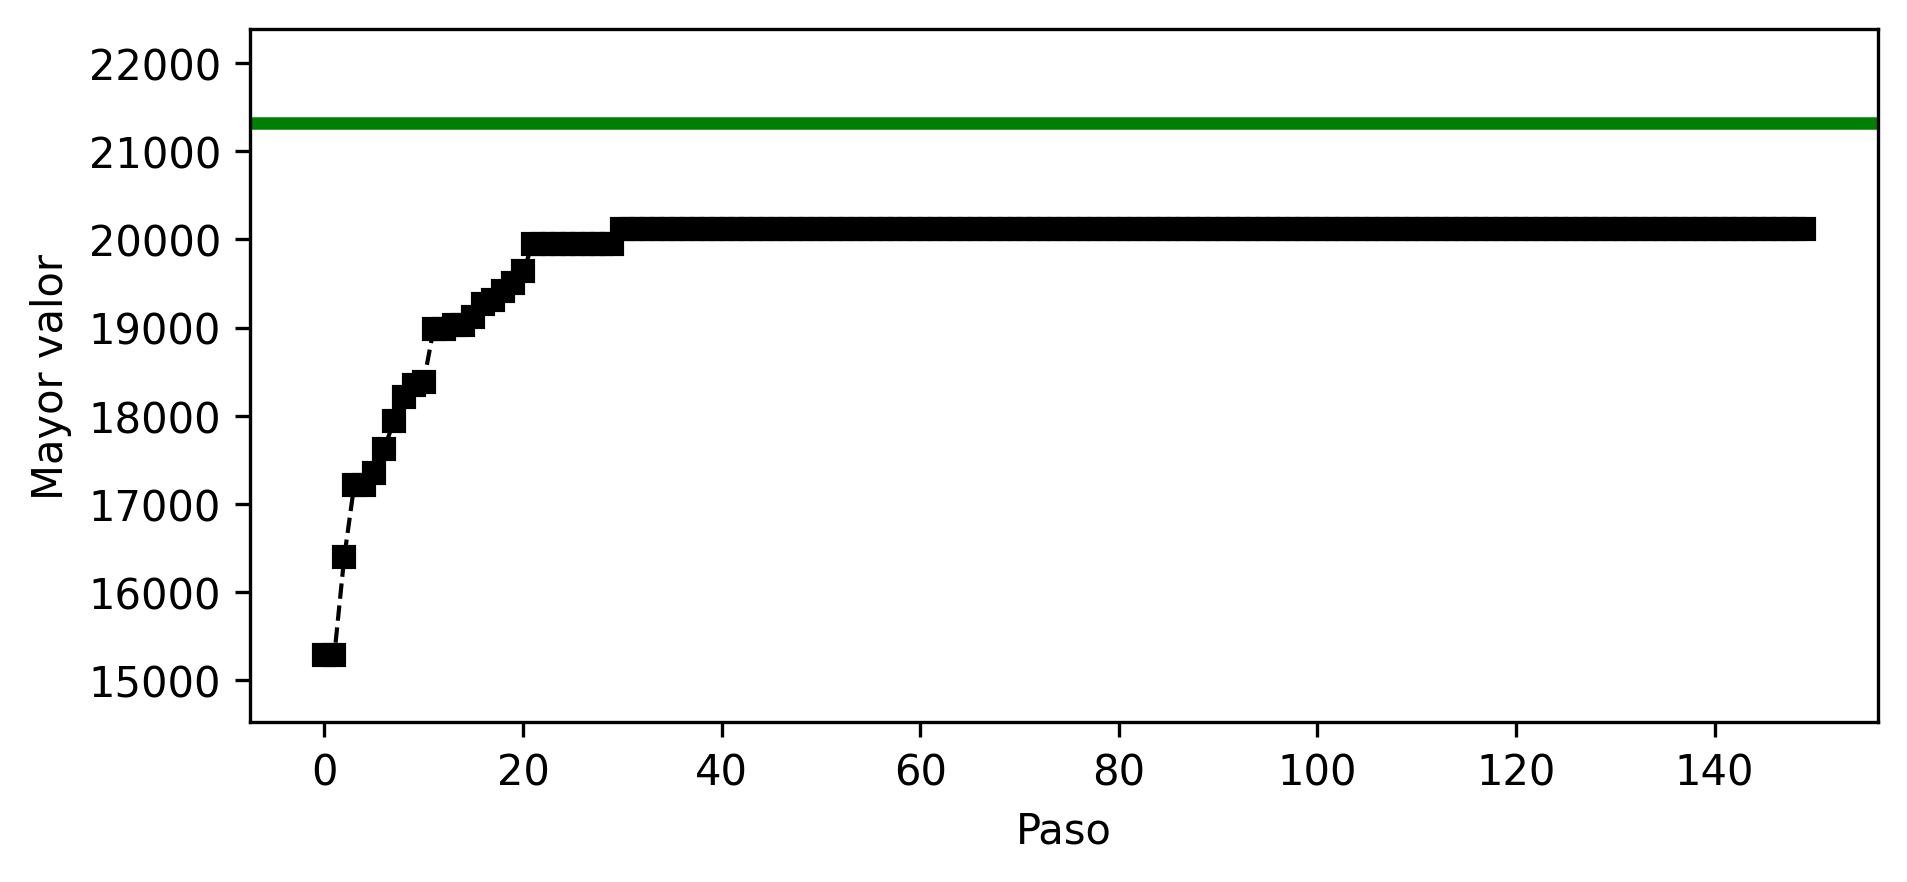
\includegraphics[width=\textwidth]{Images/p10p_I1_C1.png}
         \caption{Desarrollo del algoritmo para la combinaci\'on 1.}
         \label{fig1a}
    \end{subfigure}
    \begin{subfigure}[b]{0.49\textwidth}
         \centering
         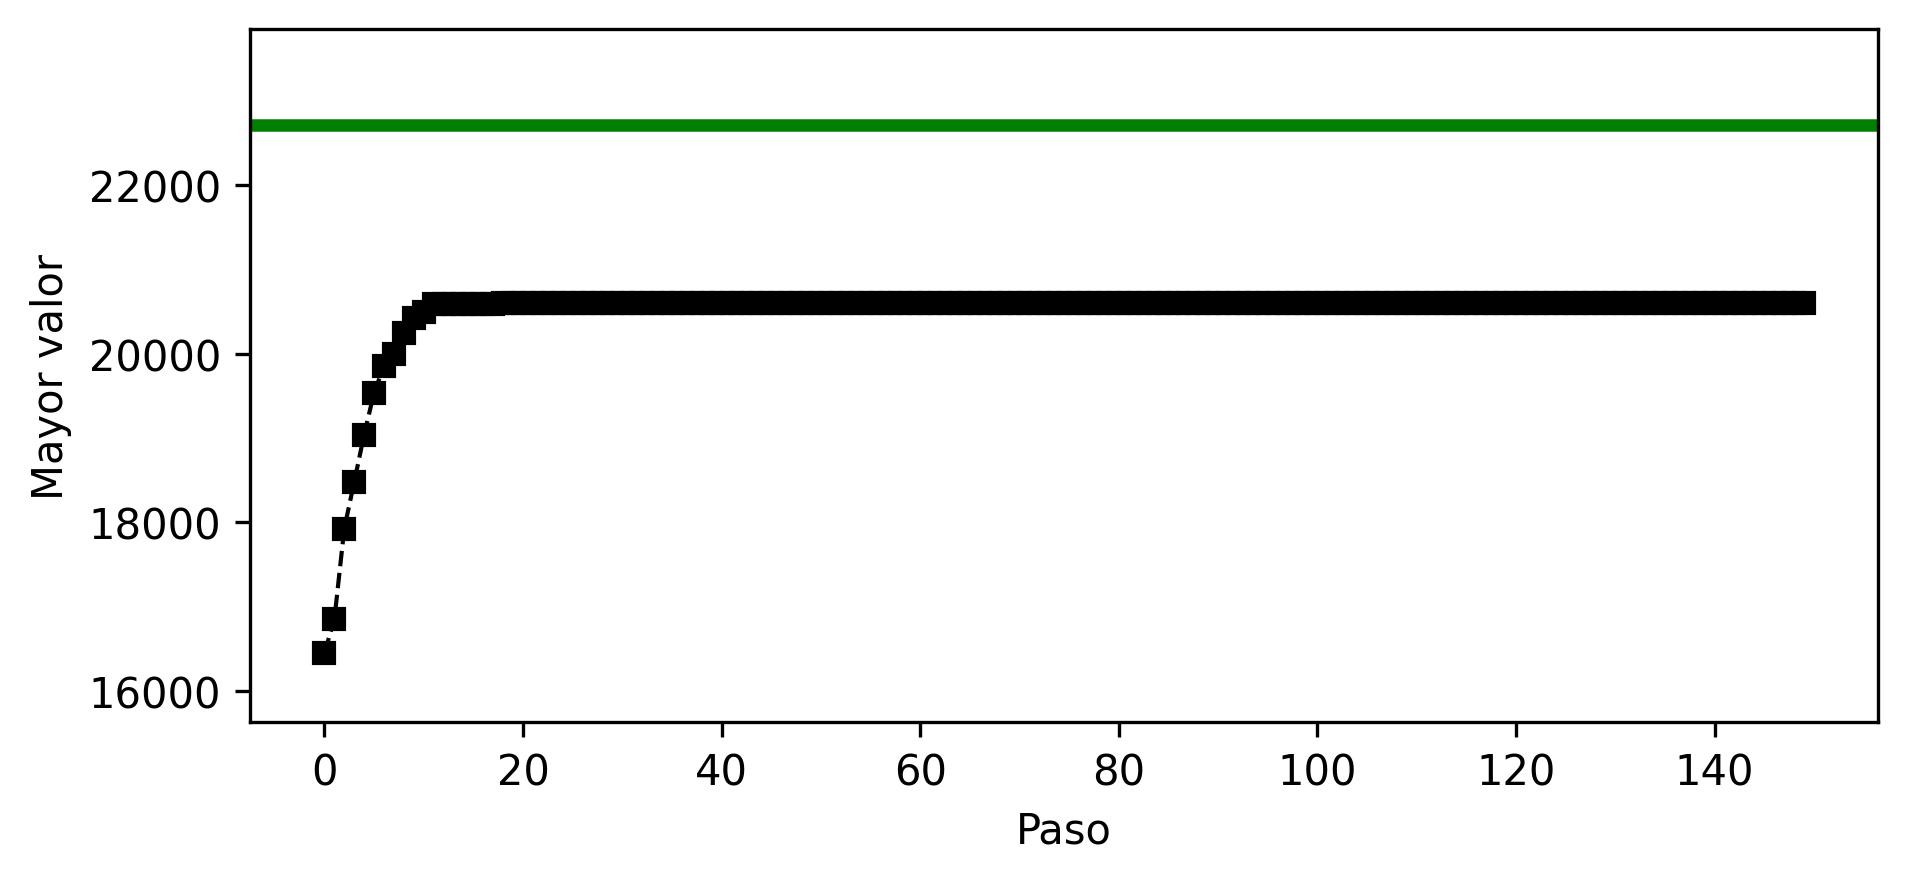
\includegraphics[width=\textwidth]{Images/p10p_I1_C2.png}
         \caption{Desarrollo del algoritmo para la combinaci\'on 2.}
         \label{fig1b}
    \end{subfigure}
    \caption{Ejemplo de iteraci\'on para la Instancia 1.}
    \label{fig1}
\end{figure}

\newpage

La figura \ref{fig2} muestra una iteraci\'on de cada combinaci\'on para la segunda instancia. Para ambos casos se puede observa c\'omo no solamente existe una mejora casi inmediata, sino que el valor m\'aximo logra alcanzar el valor \'optimo y quedarse sobre \'el. Sin embargo, se puede observar que esta instancia trabaja con valores m\'as bajos.

\begin{figure}[h]
\centering
    \begin{subfigure}[b]{0.49\textwidth}
         \centering
         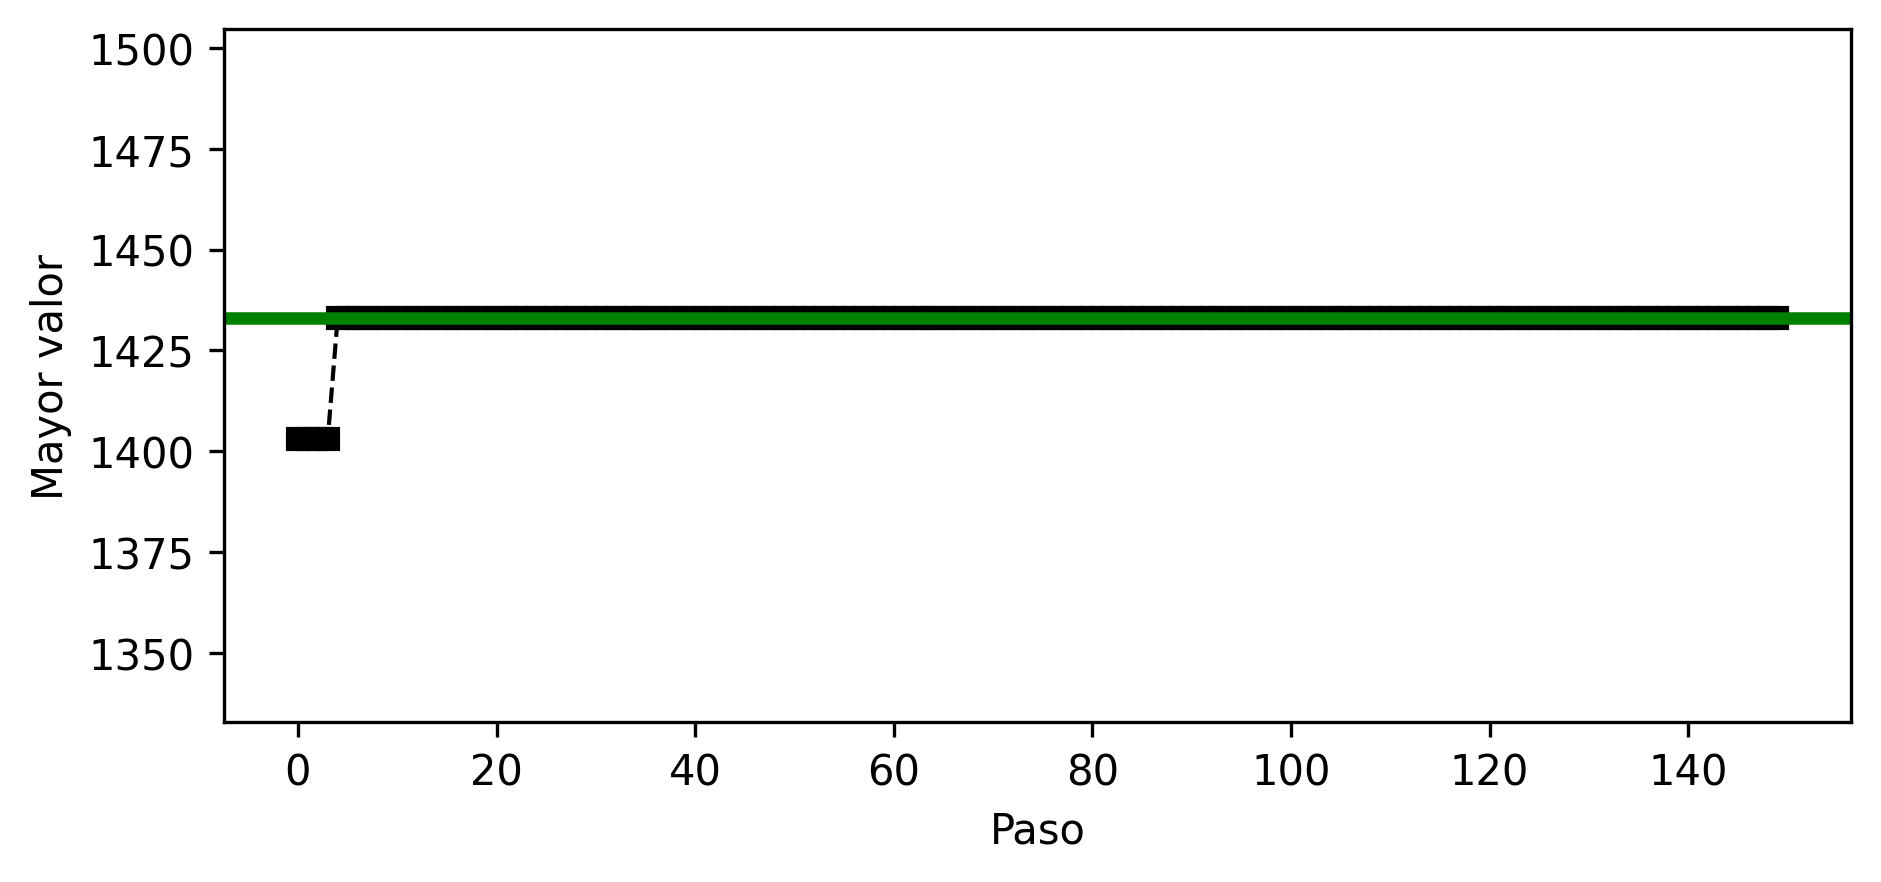
\includegraphics[width=\textwidth]{Images/p10p_I2_C1.png}
         \caption{Desarrollo del algoritmo para la combinaci\'on 1.}
         \label{fig2a}
    \end{subfigure}
    \begin{subfigure}[b]{0.49\textwidth}
         \centering
         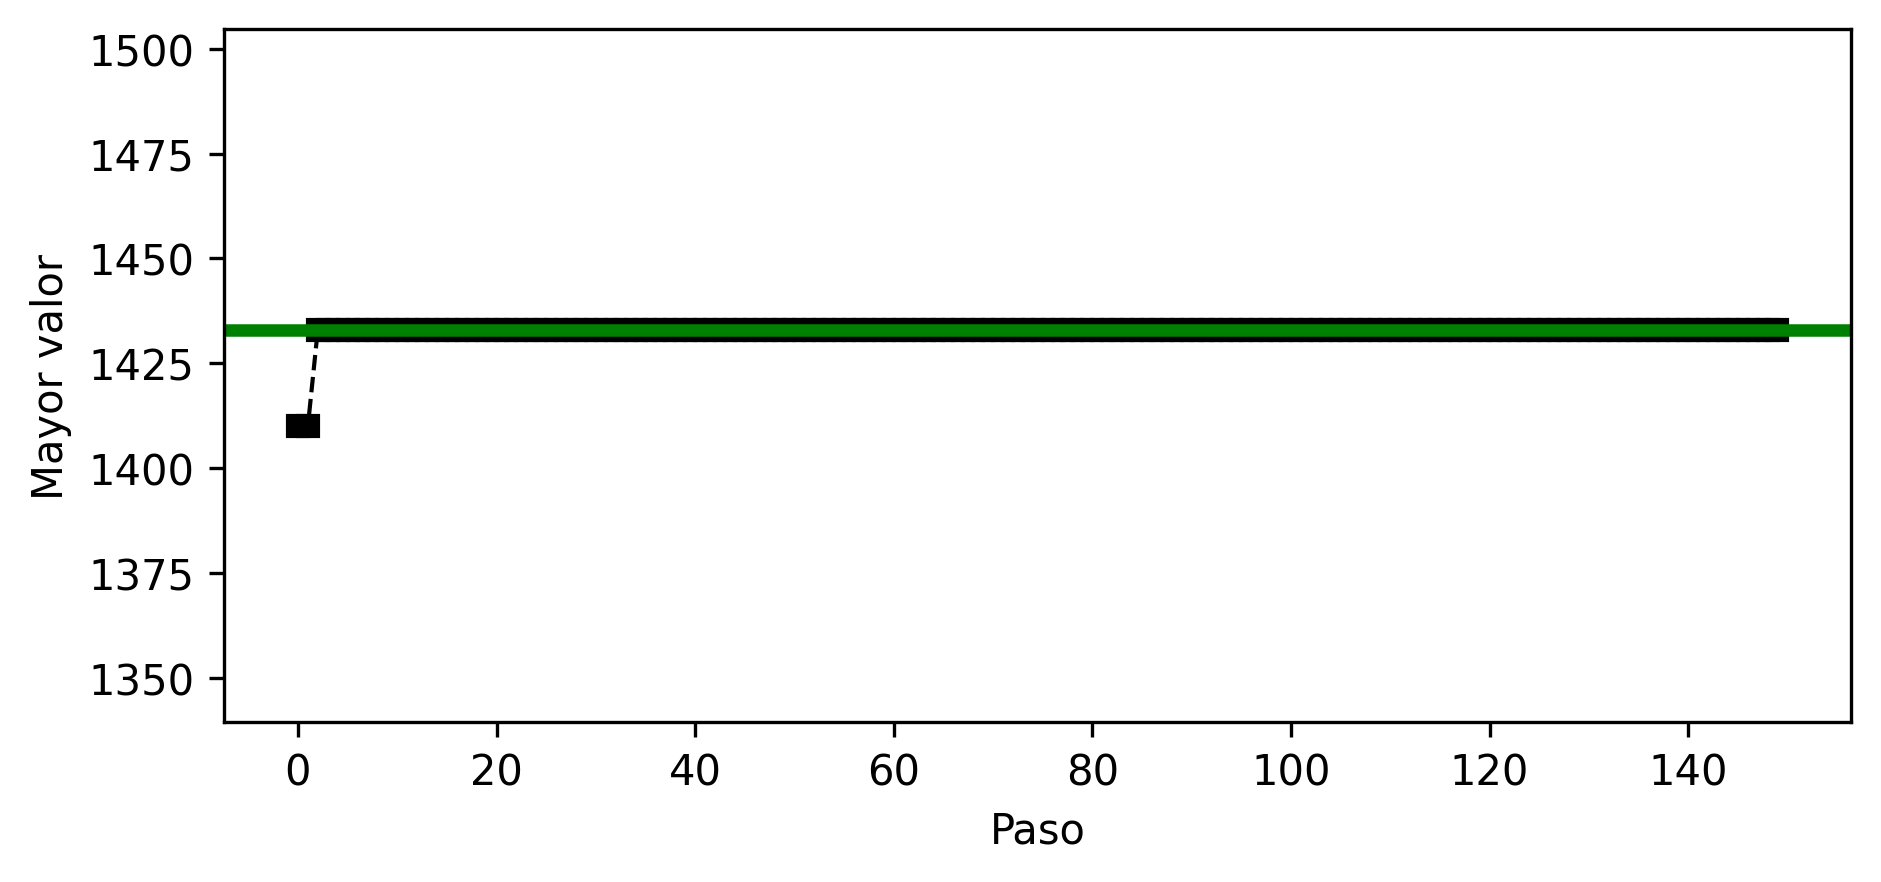
\includegraphics[width=\textwidth]{Images/p10p_I2_C2.png}
         \caption{Desarrollo del algoritmo para la combinaci\'on 2.}
         \label{fig2b}
    \end{subfigure}
    \caption{Ejemplo de iteraci\'on para la Instancia 2.}
    \label{fig2}
\end{figure}

En la figura \ref{fig3} se ven representados ejemplos de las dos combinaciones para la tercera instancia. Esta instancia puede trabajar con valores mucho mayores que las dos anteriores, en el rango de centenas de millones. Contrario al caso de la instancia 1, se puede ver c\'omo la primera combinaci\'on (figura \ref{fig3a}), presenta mejoras en ciertos intervalos y el valor m\'aximo se aproxima m\'as al \'optimo, llegando tambi\'en a estancarse casi al principio de la iteraci\'on. Por el otro lado, la combinaci\'on 2 (figura \ref{fig3b}), presenta un desarrollo m\'as gradual y la diferencia entre el valor \'optimo y el m\'aximo es m\'as grande.

\begin{figure}[h]
\centering
    \begin{subfigure}[b]{0.49\textwidth}
         \centering
         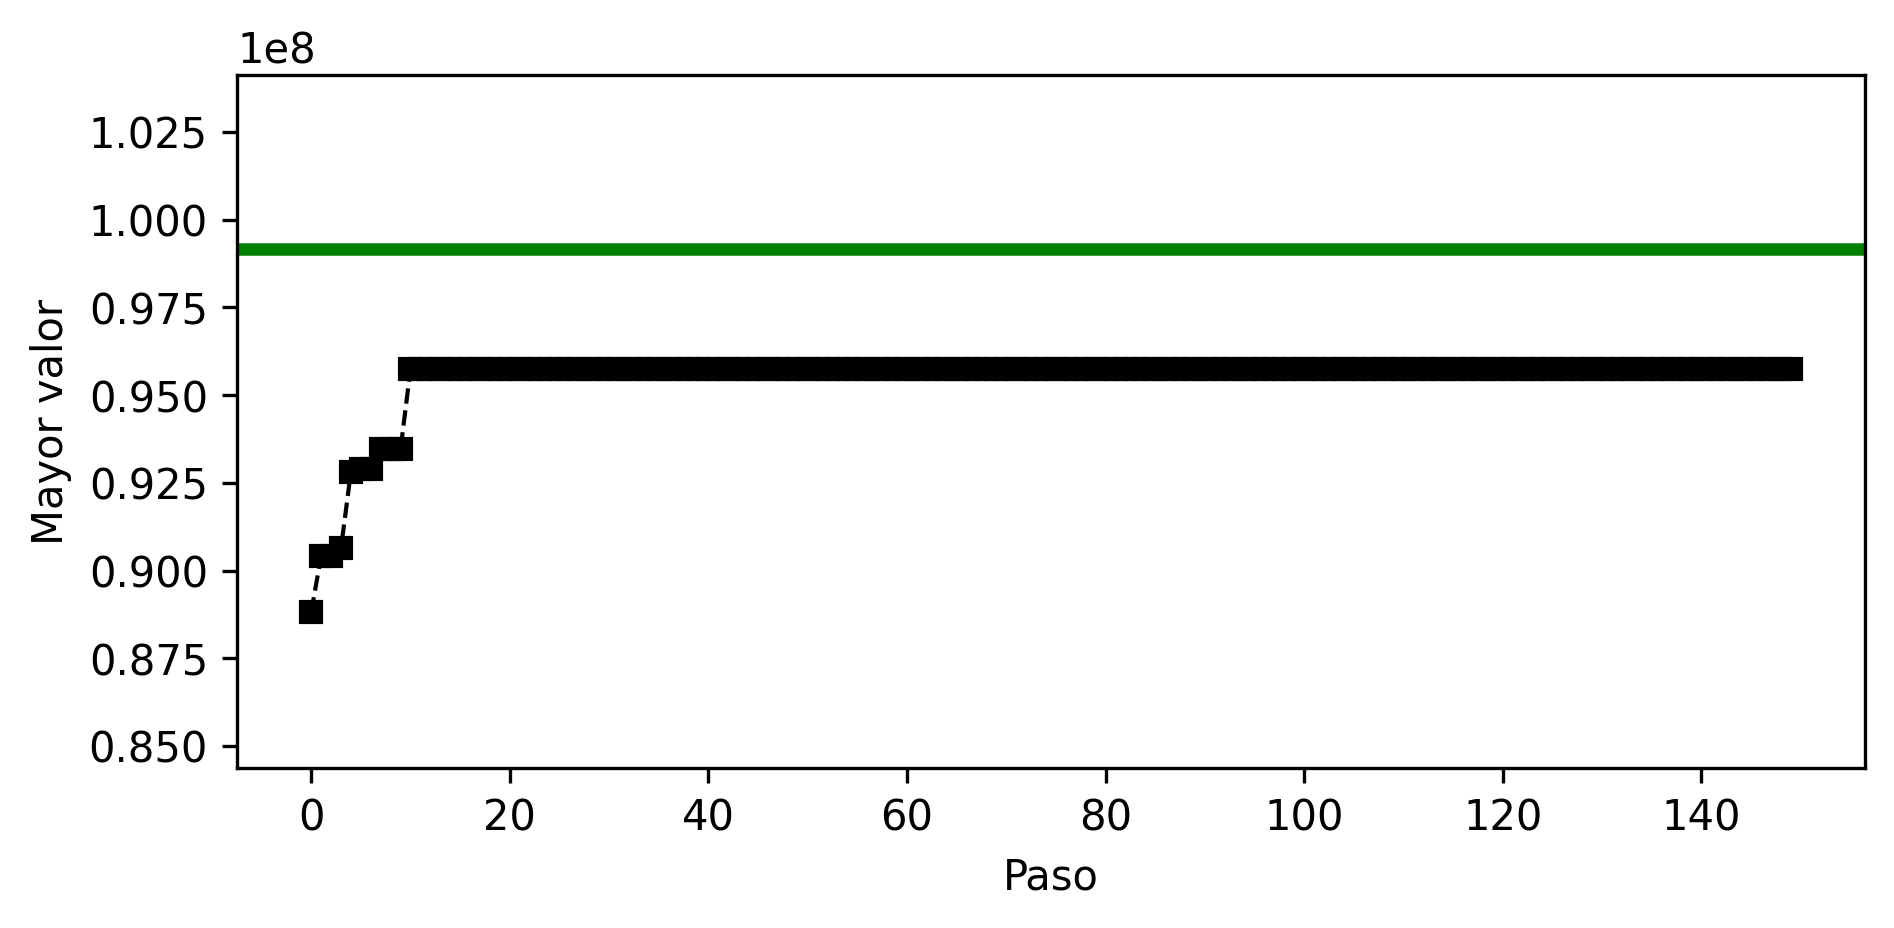
\includegraphics[width=\textwidth]{Images/p10p_I3_C1.png}
         \caption{Desarrollo del algoritmo para la combinaci\'on 1.}
         \label{fig3a}
    \end{subfigure}
    \begin{subfigure}[b]{0.49\textwidth}
         \centering
         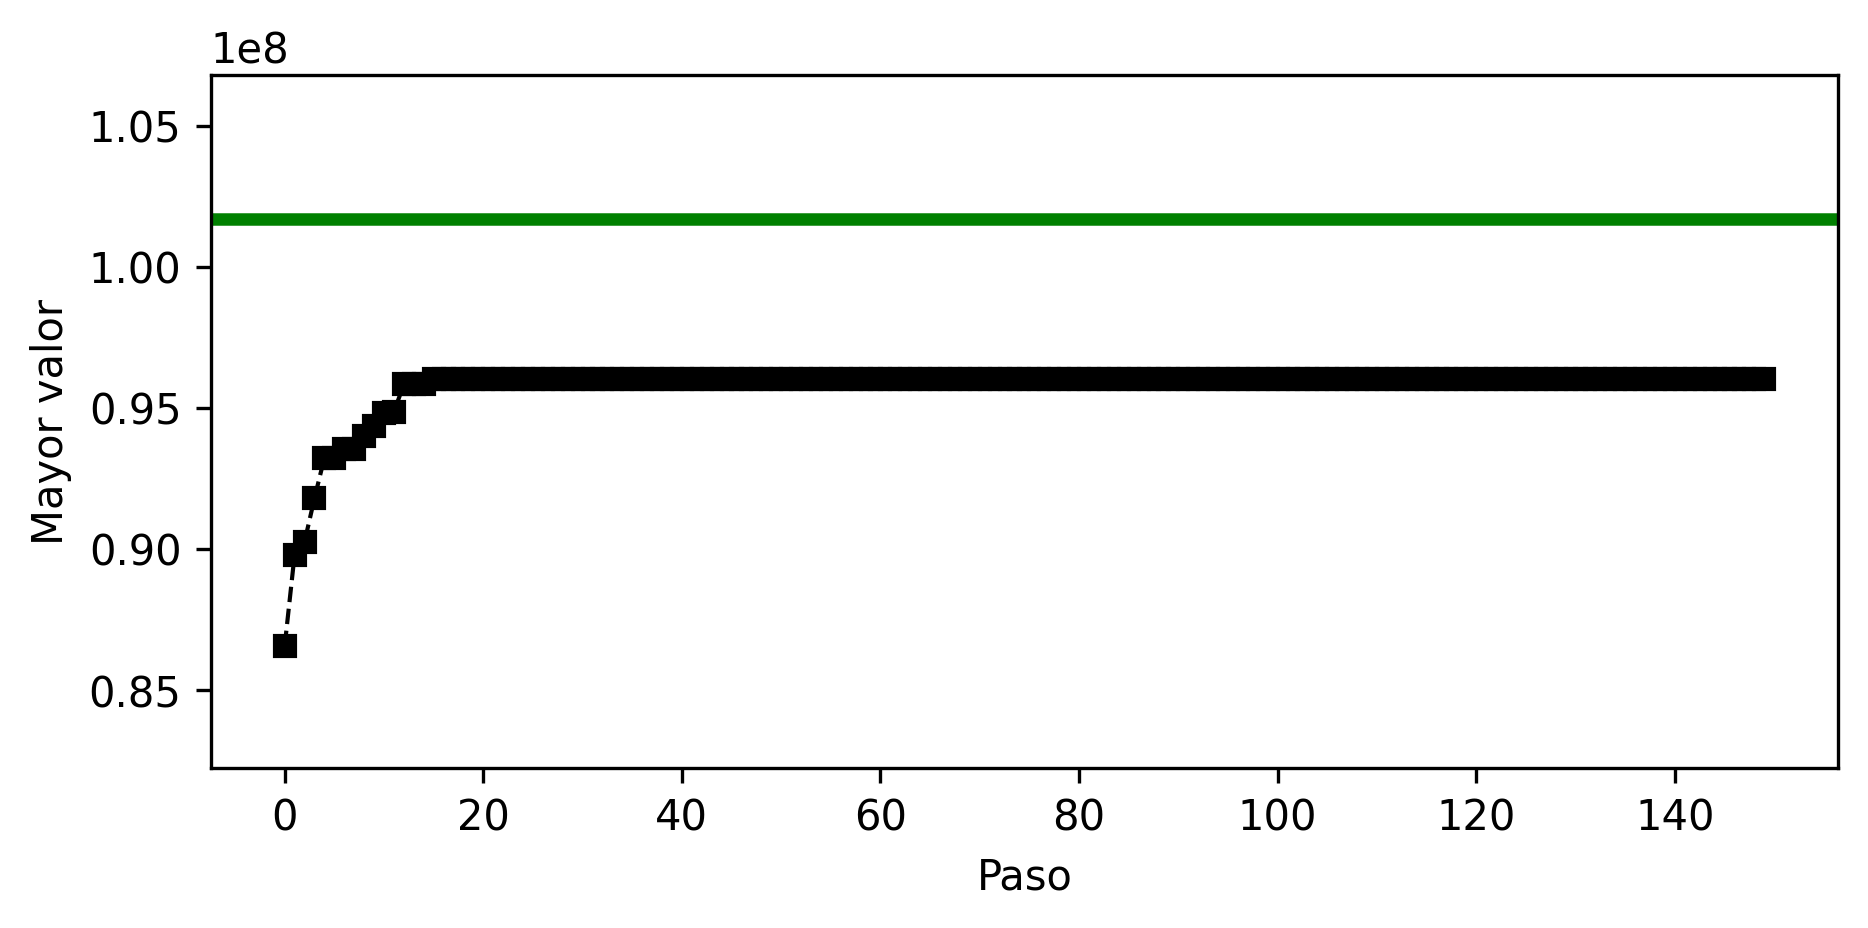
\includegraphics[width=\textwidth]{Images/p10p_I3_C2.png}
         \caption{Desarrollo del algoritmo para la combinaci\'on 2.}
         \label{fig3b}
    \end{subfigure}
    \caption{Ejemplo de iteraci\'on para la Instancia 3.}
    \label{fig3}
\end{figure}

\newpage

Para una mejor referencia visual, en la figura \ref{fig4} se han representado las mejores proporciones logradas en las 20 iteraciones de cada instancia y cada combinaci\'on en diagramas tipo viol\'in. De esta forma se puede observar la distribuci\'on que presentan, as\'i como la media para cada combinaci\'on.\\

\begin{figure}
\centering
    \begin{subfigure}[b]{0.49\textwidth}
         \centering
         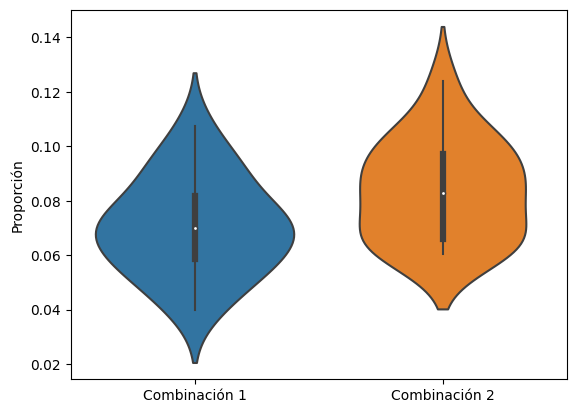
\includegraphics[width=\textwidth]{Images/p10p_I1.png}
         \caption{Distribuci\'on de ambas combinaciones para la instancia 1.}
         \label{fig4a}
    \end{subfigure}
    \begin{subfigure}[b]{0.49\textwidth}
         \centering
         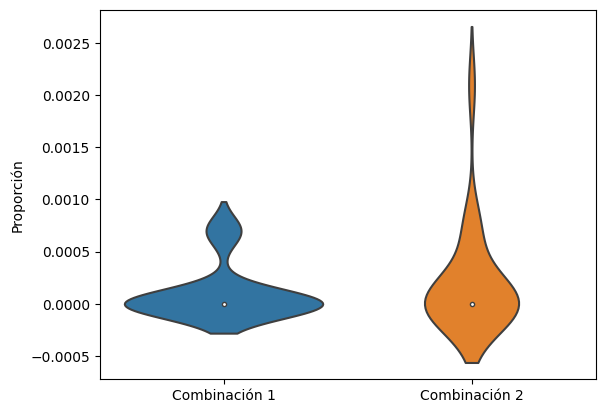
\includegraphics[width=\textwidth]{Images/p10p_I2.png}
         \caption{Distribuci\'on de ambas combinaciones para la instancia 2.}
         \label{fig4b}
    \end{subfigure}
    \begin{subfigure}[b]{0.49\textwidth}
         \centering
         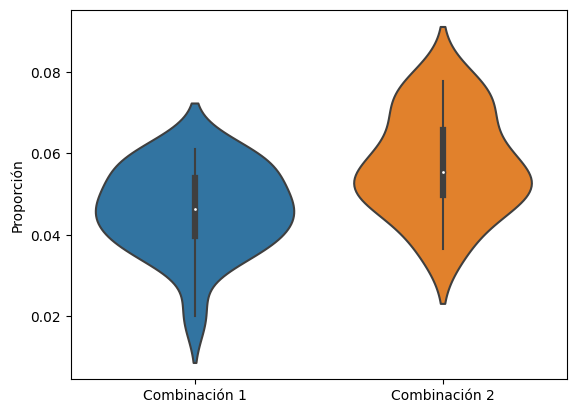
\includegraphics[width=\textwidth]{Images/p10p_I3.png}
         \caption{Distribuci\'on de ambas combinaciones para la instancia 3.}
         \label{fig4c}
    \end{subfigure}
    \caption{Distribuciones de las mejores proporciones alcanzadas para cada instancia y cada combinaci\'on.}
    \label{fig4}
\end{figure}

Se han realizado tambi\'en an\'alisis estad\'isticos de tipo ANOVA entre ambas combinaciones de cada instancia para dilucidar si existe una diferencia estad\'istica al variar la probabilidad de mutaci\'on, la cantidad de cruzamientos y el tama\~no de poblaci\'on inicial. Para la instancia 1, se ha concluido que s\'i existe una diferencia estad\'istica, ya que el resultado del an\'alisis arroja un valor $p$ mucho menor a 0.05. El valor $p$ encontrado para la instancia 2 es mayor a 0.05, por lo que se podr\'ia concluir que no existe diferencia estad\'isticamente significativa al variar los par\'ametros mencionados. En la instancia 3 tambi\'en se encuentra que hay una diferencia estad\'istica al obtener un valor $p$ menor a 0.05.

\section{Conclusiones}

Este es un ejemplo bastante b\'asico de la forma en que se puede implementar un algoritmo gen\'etico para hacer m\'as eficiente la soluci\'on de problemas complejos.\\

De los an\'alisis estad\'isticos se puede observar que, tanto para la instancia 1 como para la instancia 3, s\'i existe una diferencia en la calidad de las proporciones entre valor m\'aximo y valor \'optimo al variar los par\'ametros. Sin embargo, para la instancia 2 no existe tal diferencia en calidad. Esto podr\'ia deberse a la rapidez con la que el algoritmo llega al valor \'optimo, lo cual a su vez podr\'ia deberse a la relaci\'on exponencial entre valores y pesos cuando estos se generan.

\bibliography{tarea_10}
\bibliographystyle{plainnat}
\end{document}
